%! TEX program = luatex
\documentclass[11pt]{article}
\usepackage{textcomp}
\usepackage{graphicx,wasysym, mdframed,xcolor,gensymb,verbatim}
\usepackage{color}
\usepackage{floatflt}
\usepackage[italian]{babel}
%T1 garantisce la visualizzazione corretta del font  FiraMono usato per i codici
%con T1 i caratteri sono rappresentati a 8 bit e quindi si hanno a disposizione 256 glyphs
%la scelta migliore sare TU (unicode) ma questa � supportata solo da XeTeX e LuaTeX
\usepackage[scaled=0.8]{FiraMono}
\definecolor{verdeoliva}{rgb}{0.3,0.3,0}
\definecolor{grigio}{rgb}{0.5,0.5,0.5}
\definecolor{blumarino}{rgb}{0.0,0,0.5}
\definecolor{panna}{rgb}{0.98,0.98,0.94}
\def\lstlistingname{Listato}
\lstset{%
  backgroundcolor=\color{panna},   % choose the background color; you must add \usepackage{color} or \usepackage{xcolor}; should come as last argument
% basicstyle=\footnotesize\ttfamily,
  basicstyle=\ttfamily,
%  belowskip=-0.8 \baselineskip,
% basicstyle=\footnotesize,        % the size of the fonts that are used for the code
  breakatwhitespace=false,         % sets if automatic breaks should only happen at whitespace
  breaklines=true,                 % sets automatic line breaking
  captionpos=b,                    % sets the caption-position to bottom
  commentstyle=\color{verdeoliva},    % comment style
% deletekeywords={},            % if you want to delete keywords from the given language
% escapeinside={\%*}{*)},          % if you want to add LaTeX within your code
% extendedchars=true,              % lets you use non-ASCII characters; for 8-bits encodings only, does not work with UTF-8
% firstnumber=1000,                % start line enumeration with line 1000
  frame=single,	                   % adds a frame around the code
  keepspaces=true,                 % keeps spaces in text, useful for keeping indentation of code (possibly needs columns=flexible)
  keywordstyle=\color{blue},       % keyword style
% language=Octave,                 % the language of the code
% morekeywords={*,},            % if you want to add more keywords to the set
  numbers=left,                    % where to put the line-numbers; possible values are (none, left, right)
  numbersep=5pt,                   % how far the line-numbers are from the code
  numberstyle=\tiny\color{grigio}, % the style that is used for the line-numbers
  rulecolor=\color{black},         % if not set, the frame-color may be changed on line-breaks within not-black text (e.g. comments (green here))
  showspaces=false,                % show spaces everywhere adding particular underscores; it overrides 'showstringspaces'
  showstringspaces=false,          % underline spaces within strings only
  showtabs=false,                  % show tabs within strings adding particular underscores
  stepnumber=1,                    % the step between two line-numbers. If it's 1, each line will be numbered
  stringstyle=\color{blumarino},   % string literal style
  tabsize=2,	                   % sets default tabsize to 2 spaces
  title=\lstname%                  % show the filename of files included with \lstinputlisting; also try caption instead of title
}

\newcommand{\linuxfunction}[1]{\textcolor{blue}{function} \textcolor{purple}{#1}(}
\lstdefinestyle{linux}{
    basicstyle = \ttfamily,
    keywordstyle = \color{blue},
    keywords = {pwd,ls,mkdir,mv,rm,man,cd,cp},
    moredelim = [is][\linuxfunction]{function\ }{(}
}

\lstset{basicstyle=\ttfamily,
  showstringspaces=false,
  commentstyle=\color{red},
  keywordstyle=\color{blue}
}
\newcommand{\voto}[1]{[\textbf{#1} punti]}
\newcommand{\freccia}[1]{\vspace{1mm}\textbf{$\RHD$ #1}\\}
\def\cmu{\mbox{cm$^{-1}$}}
\def\half{\frac{1}{2}}

\voffset -2cm
\hoffset -2.5cm
%\marginparwidth 0cm
\textheight 22cm
\textwidth 17cm
%\oddsidemargin  0.2cm                                                                                         
%\evensidemargin 0.4cm                                                                                         
\parindent=0pt

\begin{document}
\pagestyle{empty}
\begin{center}
{\Large \bf  Il Sistema Linux\\[2mm]}
%{\large Canale A-C 2019-2020}
\end{center}
\vspace{4mm}
\hrule
\vspace{2mm}

\freccia{Procedura di Login}

Una volta acceso il computer e caricato il sistema operativo, l'utente esegue la procedura di Login. Il Login richiede uno username e una password. 
Per ciascun gruppo sono stati preparati degli account i cui nomi sono {\tt lcYYXX} dove  {\tt YY} sono le iniziali del docente e {\tt XX=}$0,1,\ldots, 50 $ 

\begin{lstlisting}
Username: lcng07
Password: lcng07  
\end{lstlisting}

\freccia{Cartelle e documenti}

Quando l'utente entra nel sistema gli viene assegnata un'area di disco dedicata ai propri documenti (files) che pu\`{o}essere divisa in cartelle (directories). Una directory rappresenta una divisione logica dell'area di disco. Le directories hanno un nome che segue le stesse convenzioni dei nomi dei files. Una directory pu\`{o} contenere altre directories in un albero gerarchico. Il livello pi\`{u} alto della gerarchia \`{e} rappresentato dalla directory \emph{radice} (root), rappresentata dal simbolo $/$ (slash). La radice, contiene altre directories tra cui la directory \emph{home} che contiene a sua volta le directories dei singoli utenti. L'albero delle directories si pu\`{o} navigare separando i nomi delle directories con uno il simbolo $/$.
Il percorso di una directory descrive la sua collocazione nella struttura gerarchica. Ad esempio, se la cartella \texttt{/home/} contiene la sottocartella utente1 (come nell'esempio grafico), allora il percorso della directory sar\`{a} {\tt /home/utente1/}. La stessa cosa vale se all'interno della directory ci sia un file: ad esempio, il percorso del file chiamato file1 \`{e}  {\tt /home/utente1/file1}. Si noti come le directories possano contenere sia files che altre directories (vedere Figura 1).

\begin{center}
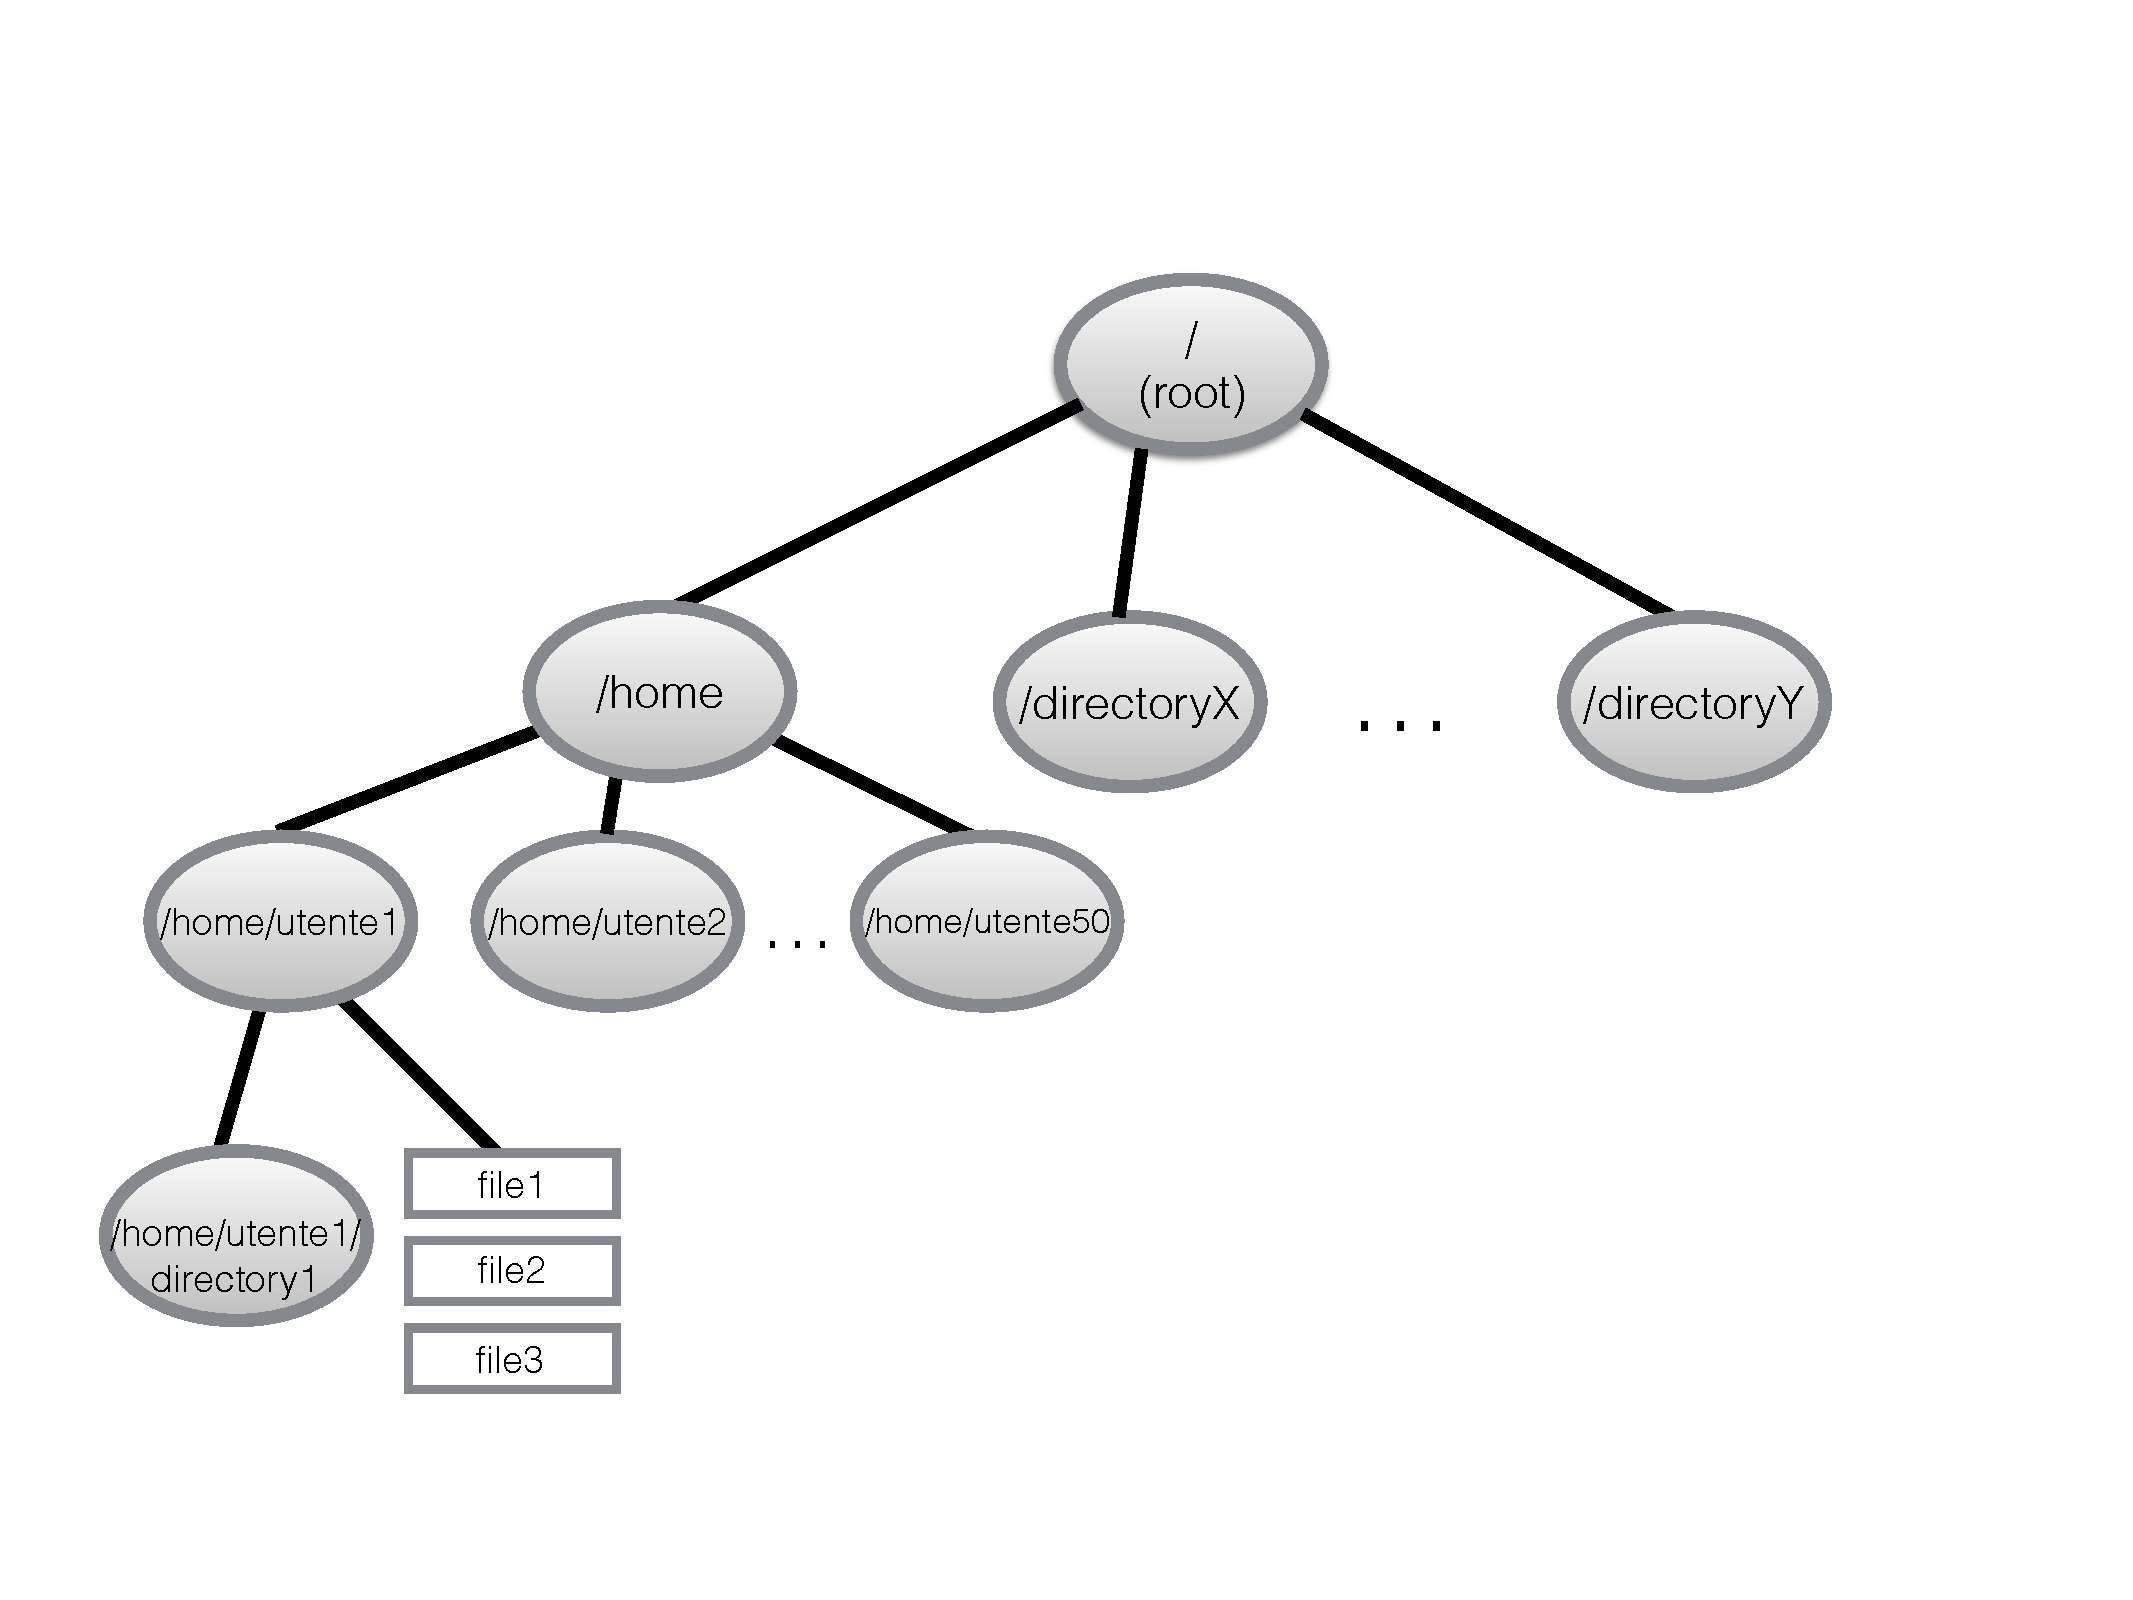
\includegraphics[width=0.75\textwidth]{Albero}
\end{center}

\freccia{La shell}

In Linux (e in UNIX) si interagisce con il sistema attraverso un programma chiamato shell che viene invocato automaticamente al Login. I comandi sono dati sotto la shell che li interpreta, li esegue e scrive il risultato su terminale. La linea comandi \`{e} caratterizzata un prompt ($\$$) e da un cursore (che generalmente \`{e} rappresentato dal carattere $\_$ o da un rettangolino lampeggiante). Nel prompt possono essere indicate alcune informazioni come ad esempio il nome dell'utente

\begin{lstlisting}[style=linux]
utente1:~$
\end{lstlisting}

\freccia{Visualizzazione della directory corrente (pwd)}

Il comando pwd (\emph{print working directory}) visualizza la posizione attuale dell'utente nella gerarchia nell'area del disco assegnata 

\begin{lstlisting}[style=linux]
utente1:~$ pwd
/home/utente1
\end{lstlisting}

\freccia{Visualizzazione dei files e directories nella directory corrente (\texttt{ls})}

Il comando \texttt{ls} (list) restituisce l'elenco dei files e delle cartelle della directory corrente. 
\begin{lstlisting}[style=linux]
utente1:~$ pwd
/home/utente1
utente1:~$ ls
directory1   file2
file1        file3
utente1:~$
\end{lstlisting}

Alla fine dell'elenco riappare il prompt, dove si pu\`{o} digitare un altro comando. Alcune opzioni utili per il comando \texttt{ls} sono:
\begin{enumerate}
\item {\tt ls -a} mostra anche i file nascosti
\item {\tt ls -l} mostra tutti i dettagli di ogni file

\end{enumerate}
Se al comando {\tt ls} si passa il nome di un file o di una directory il comando mostra solo il file o la directory indicati. Il nome si pu\`{o} esprimere usando la wildcard $*$: un carattere speciale che corrisponde a tutti i possibili caratteri. 
Per esempio 

\begin{lstlisting}[style=linux]
utente1:~$ ls -l *.pdf
\end{lstlisting}

mostra, con tutti i dettagli, la lista dei files che terminano con {\tt .pdf} . In generale tutti i comandi Unix si compongono di una parola chiave ({\tt ls}) cui seguono zero o pi\`{u} parametri ($*${\tt  .pdf} ) e/o dei modificatori ({\tt -l})  che ne alterano il comportamento di default. Per conoscere tutti i possibili usi di un comando si pu\`{o} usare il comando \texttt{man} (manuale) 

\begin{lstlisting}[style=linux]
utente1:~$ man ls
\end{lstlisting}

\freccia{Creare una nuova directory (mkdir)}

Per creare una directory, nella shell si usa il comando mkdir (make directory)

\begin{lstlisting}[style=linux]
utente1:~$ mkdir directory1
\end{lstlisting}

dove, in questo esempio, directory1 \`{e} il nome della cartella che abbiamo creato

\freccia{Spostamento in un'altra directory (cd)}

Il comando {\tt cd} (change directory) seguito dal percorso di una directory permette di spostarsi all'interno di essa

\begin{lstlisting}[style=linux]
utente1:~$ cd /home/utente1/directory1
utente1:~$ pwd
/home/utente1/directory1
\end{lstlisting}

usando il comando {\tt cd ..} si sale di un livello nella gerarchia di cartelle.
Per tornare nella directory principale ({\tt /home/utente1}) si pu\`{o} dare il comando {\tt cd $\sim$}.  infatti il simbolo $\sim$  rappresenta la propria home directory. 

\begin{lstlisting}[style=linux]
utente1:~$ pwd
/home/utente1/directory1
utente1:~$ mkdir my_dir
utente1:~$ cd my_dir
utente1:~$ pwd
/home/utente1/directory1/my_dir
utente1:~$ cd ~
utente1:~$ pwd
/home/utente1
\end{lstlisting}

Nell'esempio precedente si poteva tornare da {\tt mydir} alla home directory anche eseguendo due volte il comando {\tt cd ..} come segue
\begin{lstlisting}[style=linux]
utente1:~$ pwd
/home/utente1/directory1/my_dir
utente1:~$ cd ../../
utente1:~$ pwd
/home/utente1
\end{lstlisting}

I due punti $..$ rappresentano dunque la directory che si trova al livello superiore di quella attuale. Il punto singolo invece rappresenta la directory corrente. 

Infine un utilissimo comando \`e  \texttt{cd -} con cui si torna all'ultima cartella visitata. Ad es. 
\begin{lstlisting}[style=linux]
utente1:~$ pwd
/home/utente1/directory1
utente1:~$ cd ../directory2/my_dir
utente1:~$ pwd
/home/utente1/directory1/my_dir
utente1:~$ cd -
utente1:~$ pwd
/home/utente1/directory1
\end{lstlisting}

\freccia{Spostare e cambiare nome a files e directories (\texttt{mv})}

Per cambiare nome ad un file, si esegue un comando che "sposta" il file originale in un altro di nome diverso. Il comando da utilizzare \`{e} {\tt mv} (move):

\begin{lstlisting}[style=linux]
utente1:~$ pwd
/home/utente1
utente1:~$ ls
directory1   file2
file1        file3
utente1:~$ mv file1 nuovo_file
utente1:~$ ls
utente1:~$ directory1   file3
           file2        nuovo_file
\end{lstlisting}

Lo stesso comando pu\`{o} essere utilizzato per cambiare nome ad una cartella o spostarla in un'altra cartella 

\begin{lstlisting}[style=linux]
utente1:~$ ls
directory1   file2
file1        file3
utente1:~$ mkdir my_dir
utente1:~$ ls
utente1:~$ directory1   file1   file3
           my_dir       file2
utente1:~$ mv my_dir directory1/
utente1:~$ cd directory1/
\end{lstlisting}

Nell'esempio precedente \`{e} stata creata una cartella \texttt{my\_dir} e spostata nella \texttt{directory1}.

\begin{lstlisting}[style=linux]
utente1:~$ utente1:~$ pwd
/home/utente1/directory1/
utente1:~$  ls
my_dir
\end{lstlisting}

\freccia{Cancellare un file o una directory (\texttt{rm})}

Per cancellare un file si usa il comando \texttt{rm} (remove)

\begin{lstlisting}[style=linux]
utente1:~$ ls
directory1   file2
file1        file3
utente1:~$ rm file1 
utente1:~$ ls
directory1   file3
\end{lstlisting}

Analogamente, con lo stesso comando \`{e} possibile cancellare una directory vuota. Per cancellare una directory e tutto il suo contenuto (pensateci bene prima di usare questo comando!) si usa l'opzione  {\tt -r}

\begin{lstlisting}[style=linux]
utente1:~$ rm -r directory1
utente1:~$ ls
file1        file3
file2
\end{lstlisting}

\freccia{Copiare un file o una directory (cp)}

La copia di un file si esegue con il comando \texttt{cp} (copy) che accetta due parametri: il nome del file da copiare ({\tt file1} nell'esempio) e il nome che assumer\`{a} la copia  ({\tt copy}$\_${\tt file1}). Il comando

\begin{lstlisting}[language=bash]
utente1:~$ cp  file1 copy_file1
\end{lstlisting}

assume che  file1 esista e crea un file {\tt copy}$\_${\tt file} il cui contenuto \`{e} identico a quello di {\tt file1}. Aggiungendo l'opzione {\tt -r } \`{e} possibile copiare una directory e il suo contenuto.

\end{document}
